\chapter*{Lecture 24}
\begin{recall}{}{}
\begin{itemize}
\item Mathematical modelling of second-order ODE
\begin{itemize}
\item Spring-mass system
\end{itemize}
\item Recall make-up lecture on Thursday
\end{itemize}
\end{recall}



\section{Mathematical Modelling of second-order ODEs}

\subsection{Spring-mass system}
\begin{figure}
\centering
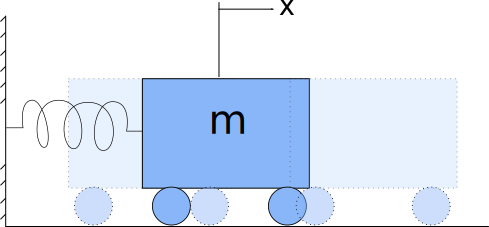
\includegraphics[width=0.6\textwidth]{figs/massSpringSystem.png} 
\end{figure}
We assume frictionless movement and that at $x=0$ the force in the spring is null.

Let's solve this problem.\\
\begin{enumerate}
\item draw free-body diagram and coordinate system\\
Variables: x (displacement) and t (time)
\item Apply physical law and setup mathematical model (Newton's second law)
\begin{equation}
\sum \vec{F}=ma=m\frac{dV}{dt}=m\frac{d^2x}{dt^2}
\end{equation}
We recall that the force of a spring is: $-kx$ (the force acts against the motion of the mass)

Our mathematical model is then:

\begin{align*}
m&\frac{d^2x}{dt^2} = -kx \qquad \text{or}\\
&\frac{d^2x}{dt^2} + \omega^2 x=0
\end{align*}
where $\omega^2=\frac{k}{m}$ where $\omega$ is the angular frequency (rad/s). [recall that the units of spring constant are $kg/s^2$, thus the units of $\omega$ are $1/s$ or $rad/s$]

\begin{align*}
\boxed{\frac{d^2x}{dt^2} + \omega^2 x=0}
\end{align*}
we have a constant coefficient homogeneous ODE.
\item Solve the ODE for $x$:\\
Auxiliary equation: $r^2+\omega^2=0$ which results in $r_1=\omega i$ and $r_2=-\omega i$ with $\alpha=0$ and $\beta=\omega$.\\
The general solution is then:
\begin{align*}
\boxed{x_g=c_1 \cos(\omega t)+c_2 \sin(\omega t)}
\end{align*}
Alternatively, we can use the trigonometric property:
\begin{align*}
\sin(A + B)=\sin(A)\cos(B)+\cos(A)\sin(B)
\end{align*}
to rewrite the above equation as:
\begin{align*}
x_g=\underbrace{E\sin(\phi)}_{c_1} \cos(\omega t)+\underbrace{E\cos(\phi)}_{c_2} \sin(\omega t)\\
x_g=E\sin(\phi+\omega t)
\end{align*}
where $E$ is the amplitude of the motion (constant) and $\phi$ the phase angle (constant).

\begin{figure}[h]
\centering
\includegraphics[width=0.5\textwidth]{figs/sin.png} 
\end{figure}
where the period $2\pi/\omega$, the amplitude $E$ and offset $-\phi/\omega$. The natural frequency of the system is $1/\text{period} = \omega/2\pi$.
\item Answer the question!
\end{enumerate}




\subsection{Spring-mass-damper system}
The system is damped:
\begin{figure}[h]
\centering
\includegraphics[width=0.6\textwidth]{figs/massSpringDamperSystem.png} 
\end{figure}

\begin{enumerate}
\item draw free-body diagram and coordinate system\\
Variables: x (displacement) and t (time)
\item Apply physical law and setup mathematical model (Newton's second law)\\

\begin{align*}
m&\frac{d^2x}{dt^2} = -kx - c\underbrace{\frac{dx}{dt}}_{v}
\end{align*}
or
\begin{align*}
\boxed{\frac{d^2x}{dt^2}+\frac{c}{m}\frac{dx}{dt} +\frac{k}{m}x =0}
\end{align*}
(inertial term) + (damping) + (spring)= (external force)\\

\item Solve for $x(t)$\\
Aux Eq. $r^2+\frac{c}{m}r+\frac{k}{m}=0$\\
We need to check what case we have:
\begin{equation*}
b^2-4ac = \frac{c^2}{m^2}-\frac{4k}{m}
\end{equation*}
which can be either greater, equal or less than zero.
All three are possible solutions and depend on the characteristics of the system.
\subsubsection{Case 1: Over-damped}
If:
\begin{equation*}
\frac{c^2}{m^2}-\frac{4k}{m}>0 \qquad \text{or} \qquad \frac{c^2}{m^2}>\frac{4k}{m}
\end{equation*}
The general solution will be:
\begin{equation*}
x_g=c_1 \exp(r_1 t)+c_2 \exp(r_2 t)
\end{equation*}
where $r_{1,2}=-\frac{c}{2m}\pm\frac{\sqrt{c^2-4km}}{2m}$. As $t\rightarrow \infty$, $x_g\rightarrow 0$.\\
The solution can be written as:
\begin{equation*}
\boxed{x_g= \exp\left(-\frac{c}{2m} t\right)\left(c_1 \exp\left(\frac{\sqrt{c^2-4km}}{2m}t\right)+c_2 \exp\left(-\frac{\sqrt{c^2-4km}}{2m} t\right)\right)}
\end{equation*}
Depending on the initial condition, we may have at most one local maximum/minimum

\subsubsection{Case 2: Critical damping}
\begin{equation*}
\frac{c^2}{m^2}-\frac{4k}{m}=0 \qquad \text{or} \qquad \frac{c^2}{m^2}=\frac{4k}{m}
\end{equation*}
The solution can be written as:
\begin{equation*}
x_g= c_1\exp\left(-\frac{c}{2m} t\right)+c_2 t \exp\left(-\frac{c}{2m} t\right)
\end{equation*}
or 
\begin{equation*}
\boxed{x_g= \exp\left(-\frac{c}{2m} t\right)\left(c_1+c_2 t\right)}
\end{equation*}

The critically damped and over-damped systems do not oscillate!



\subsubsection{Case 3: Underdamped}
\begin{equation*}
\frac{c^2}{m^2}-\frac{4k}{m}<0 \qquad \text{or} \qquad \frac{c^2}{m^2}<\frac{4k}{m}
\end{equation*}
The general solution is:
\begin{equation*}
\boxed{x_g = \exp\left(-\frac{c}{2m} t\right)\left[c_1\cos\left(\frac{\sqrt{4km-c^2}}{2m}t\right) +c_2\sin\left(\frac{\sqrt{4km-c^2}}{2m}t\right)\right]}
\end{equation*}
This solution will oscillate!

\end{enumerate}

\subsection{Forced vibration}
Now let's consider that we have an external force to the system, $F(t)$. By analysing the forces, we find:
\begin{align*}
&F_s = -kx\\
&F_d = -c \frac{dx}{dt}\\
&F(t) 
\end{align*}
\begin{figure}
\centering
\includegraphics[width=0.6\textwidth]{figs/massSpringDamperForcedSystem.pdf} 
\caption{Forced vibration spring-mass system}
\end{figure}

 Newton's Second Law becomes:
 \begin{align*}
\boxed{mx''+cx' +kx = F(t)}
\end{align*}
Above is the ODE of a spring-mass-damper system with forced vibration.

\updateinfo[November 5, 2018]